%%% Chasopys Krayany
%%% ---------------
%%% PREAMBLE
%%% ---------------
\documentclass[10pt,a4paper]{article}

% Define geometry (without using the geometry package)
\setlength\topmargin{-48pt}
\setlength\headheight{20pt}
\setlength\headsep{0pt}
\setlength\marginparwidth{-20pt}
\setlength\textwidth{7.0in}
\setlength\textheight{10.0in}
\setlength\oddsidemargin{-30pt}
\setlength\evensidemargin{-30pt}

\frenchspacing						% better looking spacing

% Call packages we'll need
\usepackage[utf8]{inputenc}
\usepackage{CJKutf8}
\newenvironment{Japanese}{%
  \CJKfamily{min}%
  \CJKtilde
  \CJKnospace}{}
\usepackage[english,ukrainian]{babel}			% languages
\usepackage{graphicx}				% images
\usepackage{amssymb,amsmath}		% math
\usepackage{multicol}				% three-column layout
\usepackage{url}					% clickable links
\usepackage{marvosym}				% symbols
\usepackage{wrapfig}				% wrapping text around figures
\usepackage[T1,T2A]{fontenc}			% font encoding
\usepackage{charter} 				% Charter font for main content
\usepackage{blindtext}				% dummy text
\usepackage{datetime}				% custom date
	\newdateformat{mydate}{\monthname[\THEMONTH] \THEYEAR}
\usepackage[pdfpagemode=FullScreen,
			colorlinks=false]{hyperref}	% links and pdf behaviour

\makeatletter\chardef\l@japanese=255 \makeatother

% Customize (header and) footer
\usepackage{fancyhdr}
\pagestyle{fancy}
\lfoot{	\footnotesize 
Спільнота українців Японії ''Краяни'' / 
\begin{CJK}{UTF8}{}
\begin{Japanese}
在日ウクライナ人コミュニティ「クラヤニイ」
\end{Japanese}
\end{CJK}
\\
		\Mundus\ \href{https://www.facebook.com/ukrainians.japan}{www.facebook.com/ukrainians.japan}	\quad
	  }
\cfoot{}
\rfoot{\footnotesize ~\\ Сторінка \thepage}
\renewcommand{\headrulewidth}{0.0pt}	% no bar on top of page
\renewcommand{\footrulewidth}{0.4pt}	% bar on bottom of page

%%% ---------------
%%% DEFINITIONS
%%% ---------------

% Define separators
\newcommand{\HorRule}[1]{\noindent\rule{\linewidth}{#1}} % Creating a horizontal rule
\newcommand{\SepRule}{\noindent							 % Creating a separator
						\begin{center}
							\rule{250pt}{1pt}
						\end{center}
						}						

% Define Title en News input
\newcommand{\Category}[1]{%
		\begin{center}	
			\Large \usefont{T2A}{kurier}{m}{n}
			\underline{#1}%
		\end{center}	
		\par \normalsize \normalfont}
		
\newcommand{\JournalIssue}[1]{%
		\hfill \textsc{\mydate \today, Випуск №1}
		\par \normalsize \normalfont}

\newcommand{\NewsItem}[1]{%
		\usefont{T2A}{iwona}{m}{n} 
		\large #1 \vspace{4pt}
		\par \normalsize \normalfont}
		
\newcommand{\NewsAuthor}[1]{%
			\hfill \textsc{#1} \vspace{4pt}
			\par \normalfont}		

%%% ---------------
%%% BEGIN DOCUMENT
%%% ---------------
\begin{document}
% Title	
% -----
\JournalIssue{1}
		
\includegraphics[width=1\textwidth]{../common_files/chasopys_logo}
%\JournalName{Краяни - часопис українців Японії}
\noindent\HorRule{3pt} \\[-0.75\baselineskip]
\HorRule{1pt}
% -----

% Front article
\begin{center}
ВІТАЄМО З ДНЕМ НЕЗАЛЕЖНОСТІ УКРАЇНИ! СЛАВА УКРАЇНІ! ГЕРОЯМ СЛАВА!
\end{center}

\SepRule
\vspace{0.1cm}

\begin{center}
\begin{minipage}[h]{0.75\linewidth}
	\begin{wrapfigure}{l}{0.61\textwidth}
		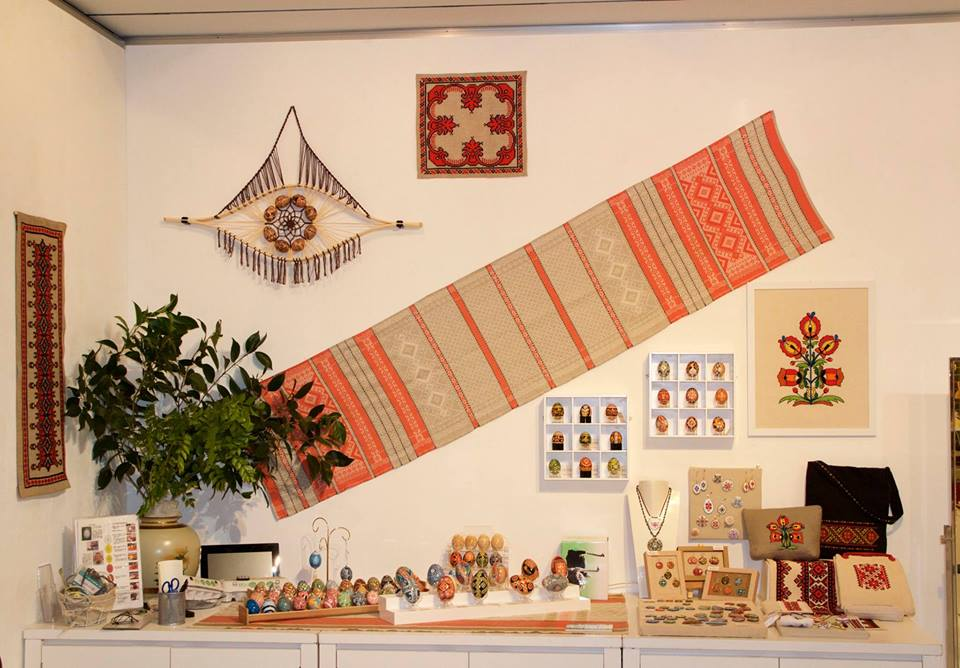
\includegraphics[width=0.62\textwidth]{images/bunkamura}
		\\	% this spacer is needed to make the text on the right fit OK
	\end{wrapfigure}
	\NewsItem{Писанки в Шібуя}
Роботи українських та японських майстринь писанкарства і вишивки були представлені на щорічній виставці ''Bunkamura Craft Collection 2015'' в Шібуя, Токіо.
\vspace{3.3cm}
\end{minipage}
\end{center}

% Page 2
\vspace{0.5cm}
	\SepRule
\vspace{0.5cm}
\begin{multicols}{3}

\vspace{1cm}
\NewsItem{Мир і війна очима дітей}
\NewsAuthor{Кіото}
		\begin{center}
			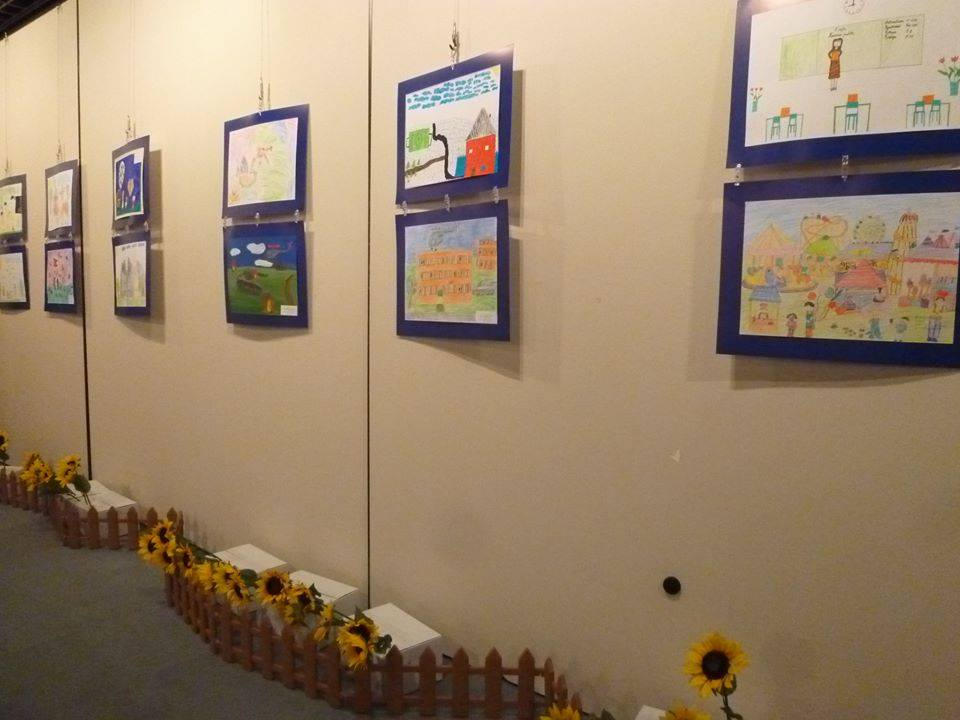
\includegraphics[width=0.8\linewidth]{images/war-and-peace}
		\end{center}
Мир і війна очима дітей - благодійна виставка робіт вихованців шкіл Донецької області з міст Слов'янськ та Краматорськ відбулась 10-11 січня у Міжнародному центрі міста Кіото.
Насичені яскравими барвами, теплом та любов'ю, дітлахи українських шкіл зобразили їхні мрії та бажання, бачення та сподівання. Багато робіт містило блакитні та жовті кольори, українську символіку, часто зображали родину, птахів та звірів, сонце, школу, мирне життя. Не зважаючи на те, якою мовою були підписані роботи: українською чи російською, з малюнків віяло теплом та сподіваннями на те, що якнайскорше відновиться мир і в Україні все буде добре.
Всім відвідувачам організатори розказали про події в Україні, про життя дітей у зоні бойових дій, демонстрували знімки учнів, відео записи їх мистецьких творів. 
Під час заходу проводився збір коштів на купівлю теплого одягу, повсякденних речей для дітей. Деякі з відвідувачів приносили теплі речі і просили їх передати в Україну.
Захід відбувся за ініціативи київського видавництва та за підтримки представника Президента України в Донецькій та Луганській області з української сторони, та за підтримки ''Товариства дружби Кіото і Києва'' та балетної школи міста Кіото - з японської. Всього було зібрано більше 700 дитячих робіт на тему ''Мир і війна очима дітей''! У виставковому центрі в Кіото в аудиторії були презентовані тільки 100 робіт учнів 16 шкіл та інтернатів Донбасу, які зобразили своє бачення миру та війни. Інша частина робіт буде представлена в Українському домі в Китаї, Великобританії та США.

\end{multicols}

\newpage

% Page 3
\Category{2015 рік}
\begin{center}
\NewsItem{3-й щорічний Мегамарш у вишиванках}	
\includegraphics[width=0.8\textwidth]{images/megamarsh}
\end{center}
\SepRule	
\begin{multicols}{3}
Дякуємо всім, хто взяв участь у 3-му щорічному Мегамарші у вишиванках у Токіо! Більше 150 українців, японців та представників інших країн світу вийшли у вишитих сорочках та з прапорами України, викликавши неабиякий інтерес у місцевого населення. Захід був організований за підтримки Посольства України в Японії та місії Української Православної Церкви Київського Патріархату ''St. Jude Ukrainian Orthodox Mission'' в місті Токіо. Цьогорічний парад був присвячений співпраці між Україною та Японією. Прапор України, що побував на Майдані у Києві, до Токіо привезла студентка з Калуша, об'єднавши українців Японії з Батьківщиною. Захід підтримав дипломатичний сектор Посольства України в Японії і надзвичайний і повноважний Посол Ігор Харченко з сім'єю. У вишиванках приєднались екс-посол Японії в Україні Саката Тоїчі з дружиною, а також відомий українознавець та генерал-полковник Українського Реєстрового Козацтва Йошіхіко Окабе. Вишиванкова хода в Токіо стала гарною традицією, а постійно зростаюча чисельність учасників та активний інтерес японців до заходу підтвердили необхідність гуртування та та створення українського осередку в Японії. Слава Україні!
\end{multicols}
 
\newpage
\begin{multicols}{3}

\vspace{1cm}
	\NewsItem{Благодійний концерт}
	\NewsAuthor{Йокогама}
		\begin{center}
			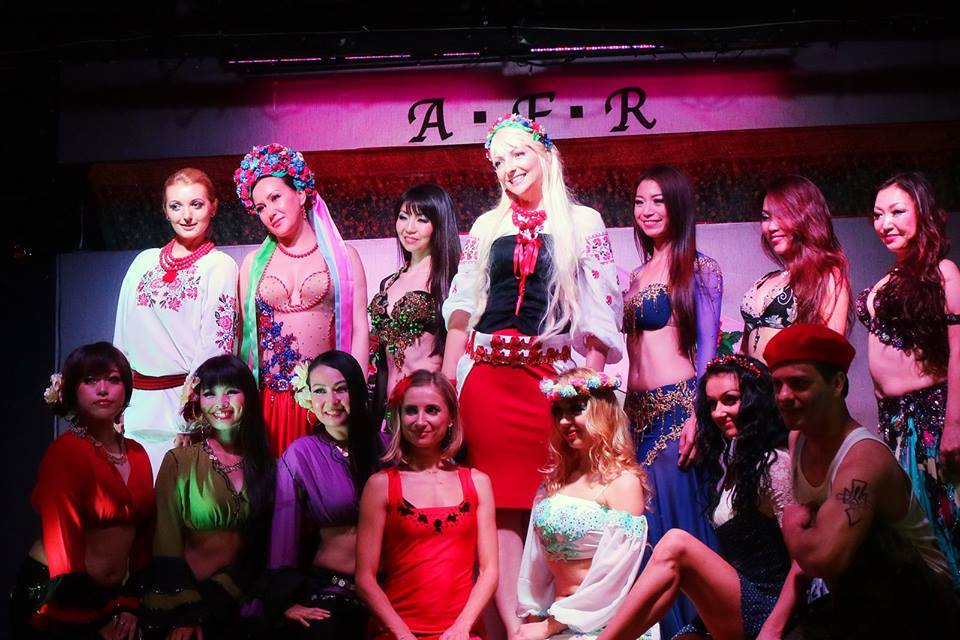
\includegraphics[width=0.8\linewidth]{images/concert}
		\end{center}
20 червня в м. Йокогама відбувся благодійний концерт на підтримку Військового Госпіталю України ''Charity For Ukraine, 2015''.
Чудовий концерт організували талановиті артисти та виконавці різних країн: Elina-star, Kateryna, Yuliya, Viktoria, Amauri Marina, Cesar Canisales, Lana, Itsuki, Erina, Emma, Eshe, Anzy, Hikari, Leila, Yasmin. Захід відбувся за підтримки Посольства України в Японії. 

\vspace{1cm}
\NewsItem{Цікаві семінари в Кансай}
\NewsAuthor{Кіото}
		\begin{center}
			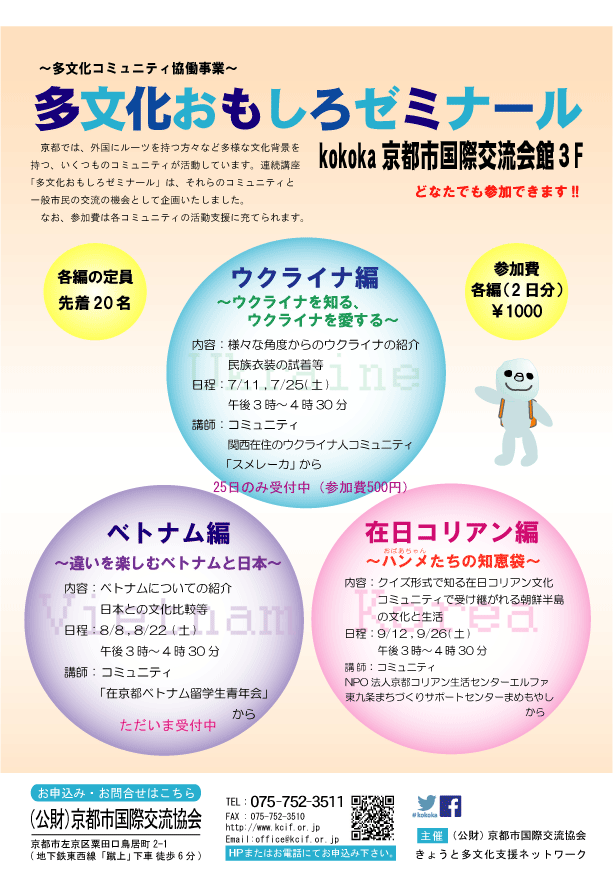
\includegraphics[width=0.8\linewidth]{images/seminary}
		\end{center}
11-го і 25-го липня у Кокока (Міжнародному Центрі міста Кіото) пройшли ''Цікаві семінари'', які організувала спільнота українців Кансаю. На семінарах, які проходили японською мовою, розповідали про основні поточні події у житті спільноти, знайомили з історією, мистецтвом і культурою нашої країни. Кошти від семінарів пішли на розвиток української громади. Також зібрали пожертви для постраждалих у війні на сході. Підготували багато цікавих презентацій. Учасники семінарів могли вдягнути український костюм, а також скуштувати українських солодощів.

\vspace{1cm}
\NewsItem{Акція-протест проти російської агресії на Донбасі та в Криму}
\NewsAuthor{Токіо}
		\begin{center}
			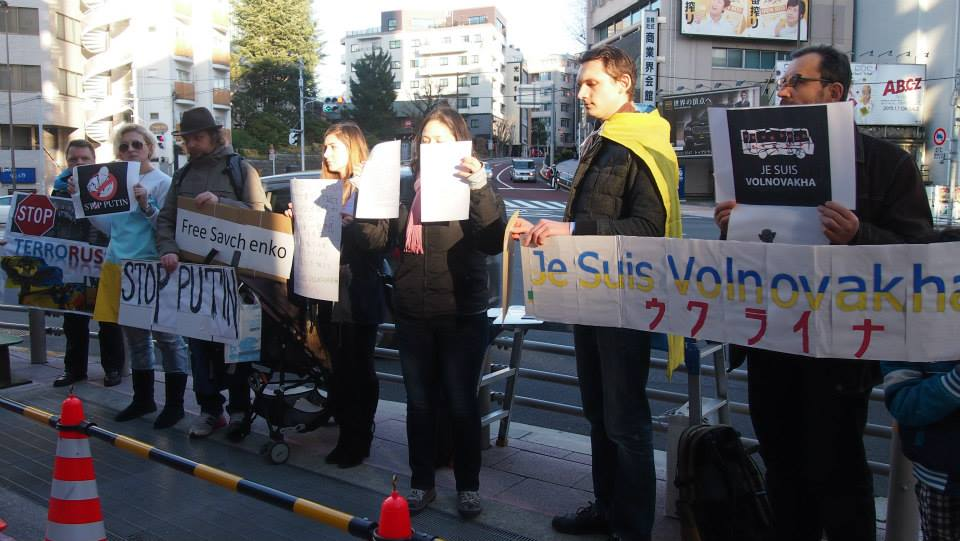
\includegraphics[width=0.8\linewidth]{images/protest}
		\end{center}
18 січня 2015 року українці Японії приєдналися до всесвітньої акції миру та солідарності із загиблими громадянами неподалік міста Волноваха. Захід відбувся біля посольства Російської Федерації в м. Токіо.
Учасники виголосили вимогу негайного припинення агресії проти України та анексії АР Крим, а також звільнення Савченко Н.В., Сенцова О.Г., інших викрадених та незаконно ув’язнених громадян України. Викладені у письмовій формі вимоги, підписані усіма присутніми учасниками акції, активісти у супроводі поліцейських віднесли до посольства Росії. Проте, як і раніше, змушені були опустити петицію у поштову скриньку. Зі сторони російської амбасади українці не отримали жодної відповіді.
Для японських ЗМІ та громадськості активісти нагадали про військові дії в Україні та смерті мирних людей, що продовжуються до сьогодні. Учасники акції нагадали про українських політичних в’язнів і голодування Савченко Н.В.
В пам’ять загиблих українських громадян, захисників України та жертв репресій учасники акції заспівали пісню «Пливе кача».
Спільно зі священником місії УПЦ КП St. Jude Ukrainian Orthodox Mission, Tokyo учасники помолились за народ України, Боже благословення та мирне врегулювання конфлікту, завершили акцію виконанням гімну України.

\vspace{1cm}
\NewsItem{Йван Канеда - диякон української церкви}
\NewsAuthor{Токіо}
		\begin{center}
			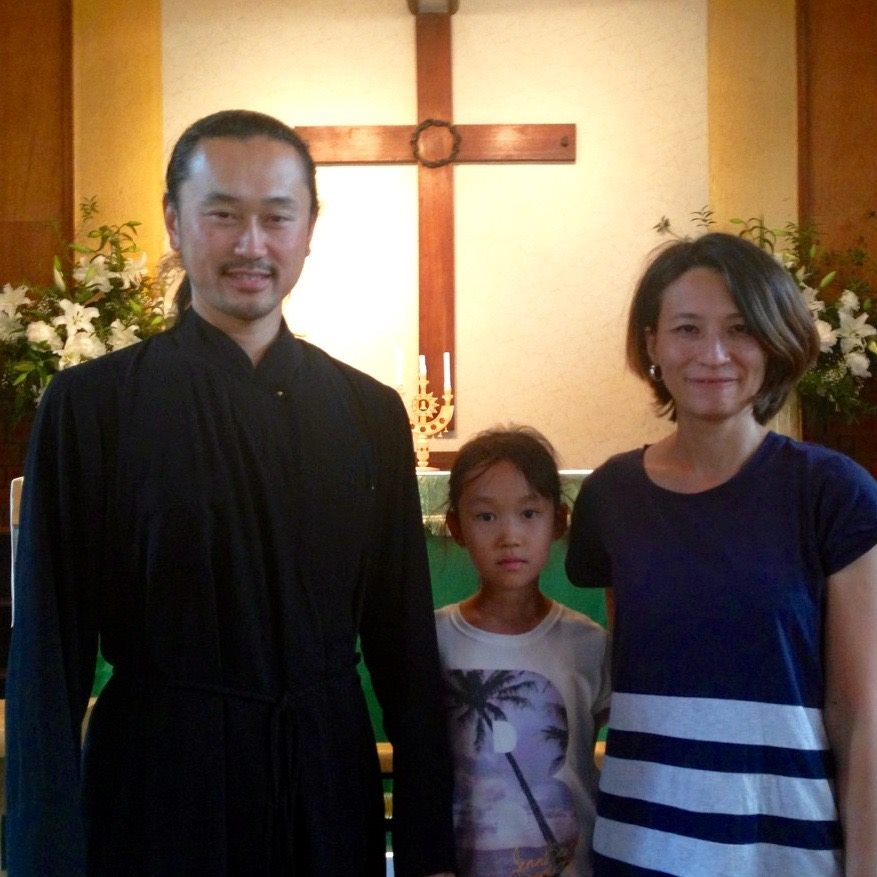
\includegraphics[width=0.8\linewidth]{images/kaneda}
		\end{center}
Разом з українською громадою в Японії, розвивається і українська православна церква в Токіо. Так, на вересень 2015 року заплановано висвячення в диякона місії Української Православної Церкви Київського Патріархату в Японії Йвана Канеди. Дасть Бог, Йван стане першим священиком-японцем нашої церкви.

\end{multicols}

\newpage

% Page 4
\Category{2014 рік}
\begin{multicols}{3}

\NewsItem{Реквієм пам'яті жертв Голодомору}
\NewsAuthor{Токіо}
		\begin{center}
			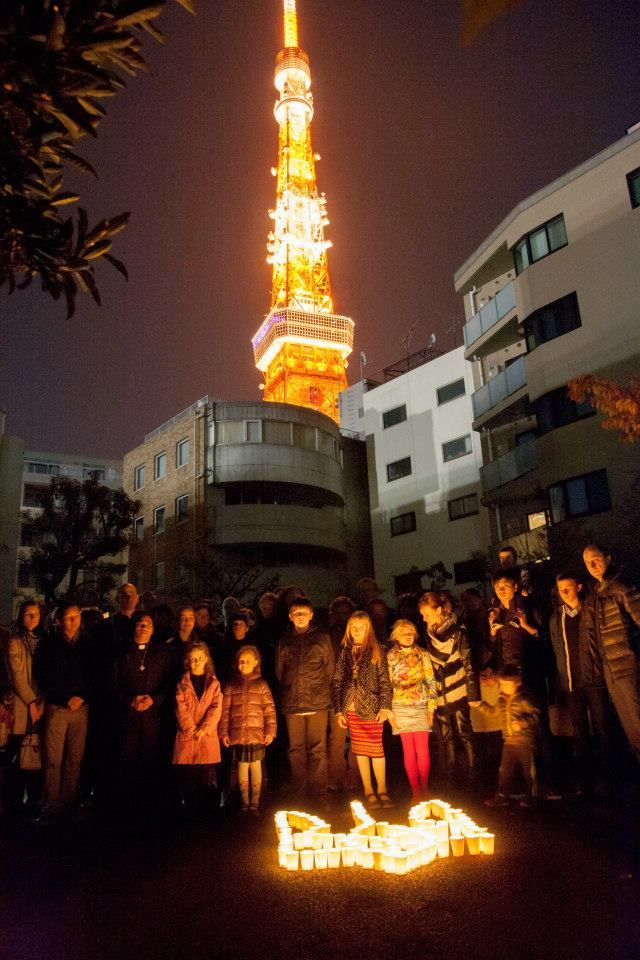
\includegraphics[width=0.8\linewidth]{images/rekviem}
		\end{center}
В Токіо 23 листопада 2004 року відбувся поминальний реквієм пам'яті жертв Голодомору в Україні, а також запалення свічок, викладених у формі національного гербу в пам'ять Героїв України, полеглим на Майдані, збір благодійної допомоги бійцям в Україні.
Близько 50 українців та їх друзів, а також дипломатичний корпус Посольства України в Японії взяли участь у поминальній службі пам'яті жертв Голодомору, організованій місією Української Православної Церкви Київського Патріархату (St. Jude Ukrainian Orthodox Mission, Tokyo). У заході також взяли участь Посол України в Японії Ігор Харченко, представники духовенства Римо-католицької та Англіканської церкви Японії.
На заході було багато присутніх дітей і у своєму зверненні до мирян, настоятель УПЦ КП отець Павло Королюк приділив увагу важливості виховання дітей, їх навчанню подій та історії, яка б вона не була гіркою та важкою; адже знаючи правду про події вони будуть розуміти зло та біль, які є у світі та зможуть захистити себе в майбутньому.
Посол України в Японії І. Харченко у своєму зверненні зазначив, що сьогодні в Україні втрачають людей тому, що режим, який в мирний час виморював українців голодом, сьогодні вбиває, сподіваючись, що може схилити, але українці пам'ятають про всіх загиблих під час Голодомору і тих, які загинули нещодавно тому, що відчувають силу і продовжують боротись; Україна й українці обов'язково переможуть.
У другій частині українська громада в Японії ''Краяни'' та всі присутні запалили 120 свічок та виклали їх у формі гербу України, що палав у центрі столиці Японії поруч з Токійською вежею.
Для допомоги бійцям Добровольчого українського корпусу було зібрано та передано 12800 гривень.
Українці Японії та місія УПЦ КП вдячні вірянам церкви Святого Альбана Англіканської церкви в Токіо за безкоштовне надання приміщення для проведення панахиди, а також регулярних Богослужінь.

\vspace{1cm}
\NewsItem{Дитячий український фестиваль в Кіото}
\NewsAuthor{Кіото}
		\begin{center}
			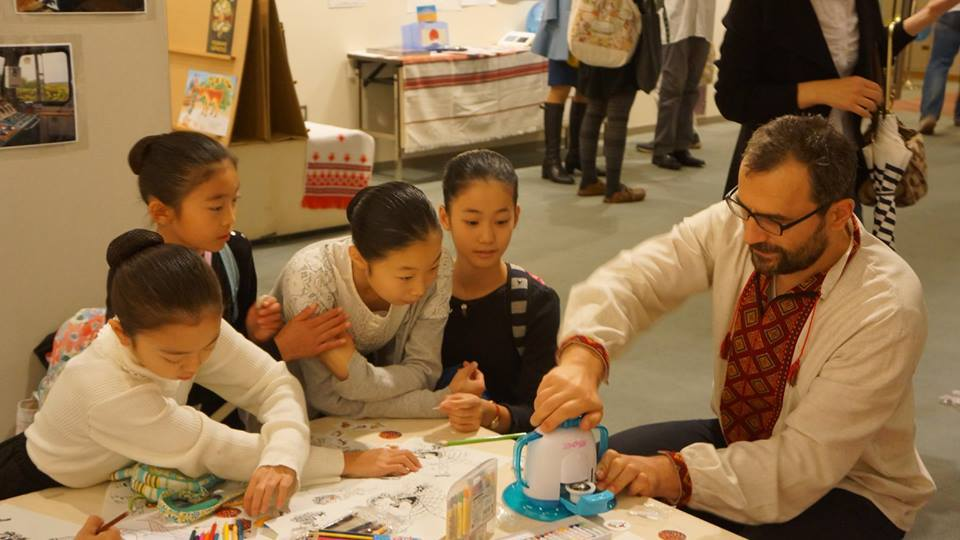
\includegraphics[width=0.8\linewidth]{images/kids-fest-kioto}
		\end{center}
В японському місті Кіото 8-9 листопада відбувся дитячий український фестиваль ''Україна. Запрошення до казки'', організований спільнотою українців, що проживають у Японії у регіоні Кансай.

На осінньому українському фестивалі в м. Кіото особливу увагу приділили японським дітям та їхньому знайомству з Україною. Для найменших був організований показ українських мультфільмів з японськими субтитрами, ігри, вікторина, виставка дитячих книжок і малюнків українських дітей. Разом з японськими гостями читали дитячі казки про ''Солом'яного бичка'', ''Рукавичку'' та інші.

Під час заходу кожен міг самостійно виготовити браслет з жовто-блакитних стрічок або значок з українською символікою, розмалювати писанку, виготовити ляльку-мотанку, а також повчитися вишиванню. Японцям представили український національний одяг, тож кожен бажаючий міг одягнутись в українське вбрання. Переможці вікторини та всі маленькі гості отримали солодкі подарунки.

У другий день фестивалю вихованці балетної школи ''Терада'' виконали українські народні танці, а також номери класичного українського балету.

На фестивалі також збирали кошти для родин з дітьми зі східних регіонів України, які наразі перебувають у Києві і якими опікується благодійна організація ''Реабілітаційний центр Шпиталь Майдану''. На потреби проекту ''Перинатальний центр'' зібрано 35000 йєн.

''Ми отримали багато позитивних відгуків від наших відвідувачів, побажання успіхів. Хоча ми зараз далеко від нашої Батьківщини, наші серця належать Україні. Ми щиро бажаємо нашій країні миру, злагоди і добробуту. Впевнені, що наша діяльність стане краплинкою у справі поширення зацікавленості японців до України і створенню більш тісних дружніх стосунків між Україною і Японією, сприятиме налагодженню зв’язків між членами української спільноти в Японії. Ми сподіваємося на подальшу підтримку і активну участь усіх, хто має до цього зацікавленість'', – зазначила одна з організаторів заходу Олена Сігал.

Зазначимо, раніше, у квітні, громадою в Кіото був проведений культурний захід ''Молимося за Україну'', який відвідали близько 1300 осіб.

\end{multicols}

\newpage

% Page 5
\begin{multicols}{3}

\NewsItem{Фестиваль ''Український день''}
\NewsAuthor{Йокогама}
		\begin{center}
			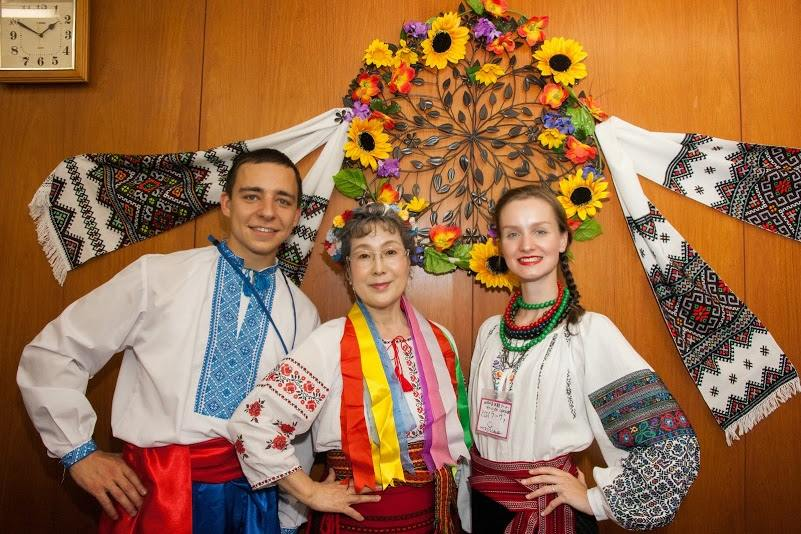
\includegraphics[width=0.8\linewidth]{images/ukr-day-fest}
		\end{center}
Відбувся ще один незабутній день в житті української спільноти в Японії!
Захід відвідало близько 500 чоловік: українці, японці, росіяни, французи, індійці, та громадяни інших країн. До учасників та гостей з вітальним словом звернувся Надзвичайний і Повноважний Посол України в Японії Ігор Харченко.
Програма заходу включала класи з писанкарства та виготовлення ляльки-мотанки, української пісні та танцю, відвідувачі вчилися азам української мови. Читалися лекції про українську культуру, мову та традиції. Популярністю серед малечі користувався дитячий куточок і куточок українських мультфільмів, а серед дорослих - куточок ''Фото з красунею та красенем''.
Працював український ресторан, де гості могли скуштувати традиційну українську кухню і звичайно ж, традиційний борщ, а також скуштувати вина та цукерок ''Рошен''. 
На закінчення свята гості відвідали концерт.
В концерті взяли участь бандуристка Kateryna, дітки-учні української школи ''Джерельце'' міста Токіо, ансамбль фольклорної музики ''Tama Linda'', аматори та професійні виконавці. Фінальним музичним номером концерту стало виконання пісні ''Господи, помилуй нас''.
Організаторами свята виступили українці, активні учасники української громади Японії — мешканці Токіо, Йокогами, префектури Сайтама і навіть віддаленого Кіото; батьки та діти — учні української школи ''Джерельце''. Особливої подяки заслуговує пан Маокі Сато, якому фестиваль завдячує наданим для свята приміщенням.
Кошти, зібрані від проведення класів, продажу українських сувенірів та української кухні передаються на допомогу воїнам, постраждалим від війни в Україні.

\vspace{1cm}
\NewsItem{Український куточок на міжнародному фестивалі в Токай}
\NewsAuthor{Токай, Аічі}
		\begin{center}
			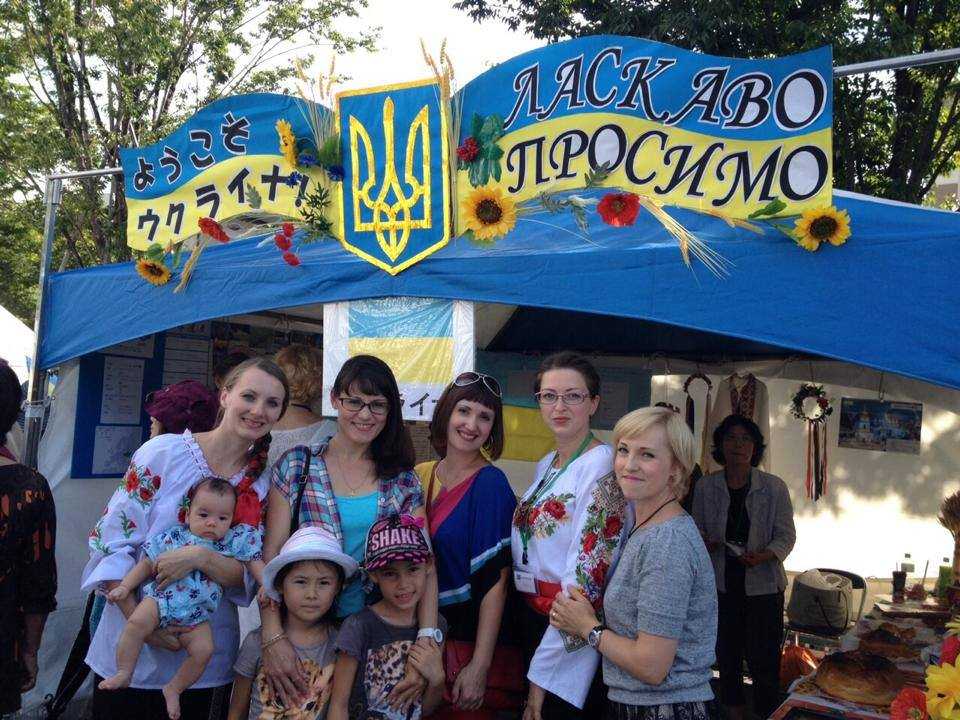
\includegraphics[width=0.8\linewidth]{images/tokai-fest}
		\end{center}
21 вересня 2004 року, в містечку Токай, неподалік міста Нагоя, відбувся фестиваль міжнародної співпраці, де Україна вже другий рік поспіль гідно представлена!

\vspace{1cm}
\NewsItem{''Інвестиції в Росію - це фінансування тероризму!''}
\NewsAuthor{Токіо}
		\begin{center}
			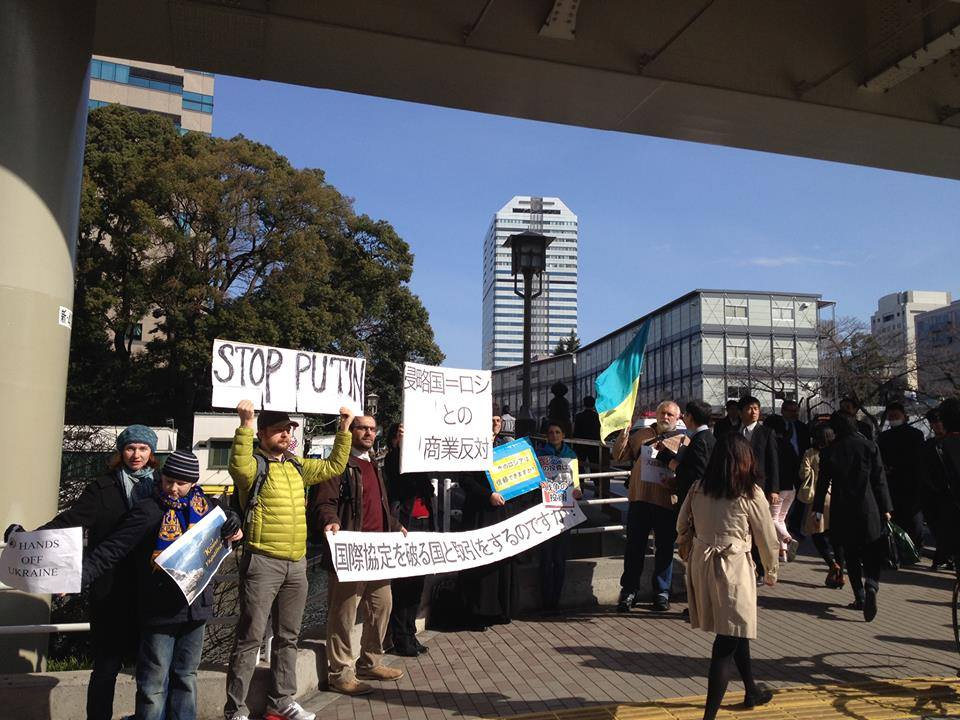
\includegraphics[width=0.8\linewidth]{images/business-forum}
		\end{center}
Сьогодні в Токіо українці в Токіо зустрічали всіх учасників 6-го російсько-японського бізнес форуму з закликами про ненадійність північного партнера. Однією з головних ідей, які хотіли донести учасники протесту - це те, що інвестуючи в російський бізнес, японська сторона може стати інвестором війни.
Подія висвітлювалась на національному каналі NHK.

\vspace{3cm}
\NewsItem{2-й Мегамарш у вишиванках}
\NewsAuthor{Токіо, Ґінза}
		\begin{center}
			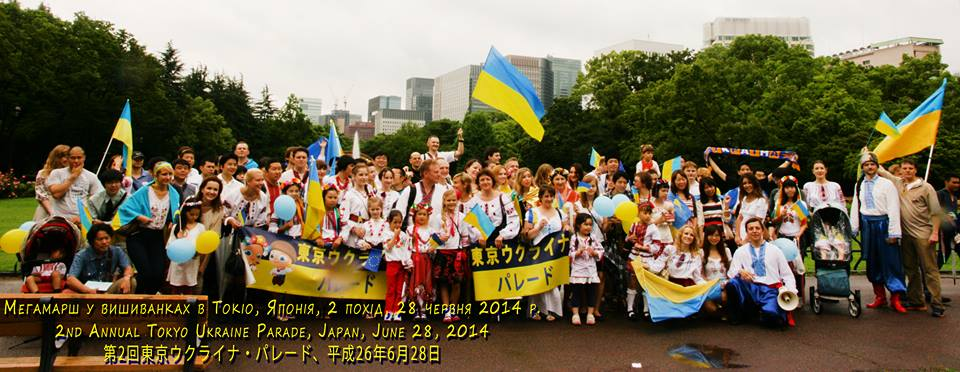
\includegraphics[width=0.8\linewidth]{images/megamarsh2004}
		\end{center}
Дякуємо кожному, хто зробив можливим проведення другого походу Мегамаршу у вишиванках в Токіо! Сьогодні до нас приєднались японці, громадяни інших країн та показали любов до нашої Батьківщини, одягнувши різнобарвні вишиванки, співаючи українських пісень, або просто приєднались до урочистої ходи. Сьогодні ми показали нашу Єдність, Гідність, Дух! Слава Україні! Слава Японії!

\vspace{1cm}
\NewsItem{День жалоби за полеглими на Майдані}
\NewsAuthor{Токіо}
		\begin{center}
			
\includegraphics[width=0.8\linewidth]{images/den-zhaloby}
		\end{center}
23 лютого - День жалоби за полеглими на Майдані. У ці трагічні дні ми, українці у Японії, не можемо залишатися осторонь того, що відбувається у нас на Батьківщині.
За проханням Посла України у Японії Ігоря Харченка сьогодні у Токіо в Українській Православній Церкві Київського Патріархату відбулася панахида за загиблими під час останніх подій у Києві, за безвинно загиблими членами Небесної Сотні.
Після панахиди були зібрані пожертви.Загальна сума пожертв склала 134 тисячі єн та 50 ам. доларів. Ця сума буде перерахована на рахунок неприбуткової організації «Разом» на вищевказані цілі.
Ми дуже вдячні отцю Павлу Королюку за організацію і проведення служби, та всім, хто знайшов час для підтримки співвітчизників у цей нелегкий час.
Разом переможемо. Слава Україні!
\end{multicols}

\newpage

\begin{center}
\NewsItem{Акція ''Українці Японії проти диктатури та державного терору'', парк Уено}	
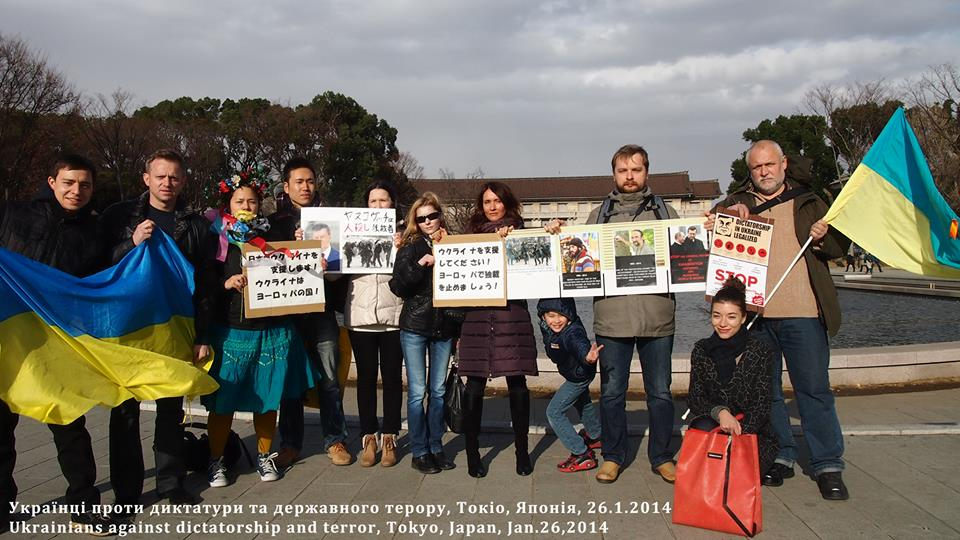
\includegraphics[width=0.8\textwidth]{images/nodictatorship}
\end{center}
\SepRule	
\begin{multicols}{2}

\NewsItem{Молитва за загиблих на Майдані}
\NewsAuthor{Токіо}
		\begin{center}
			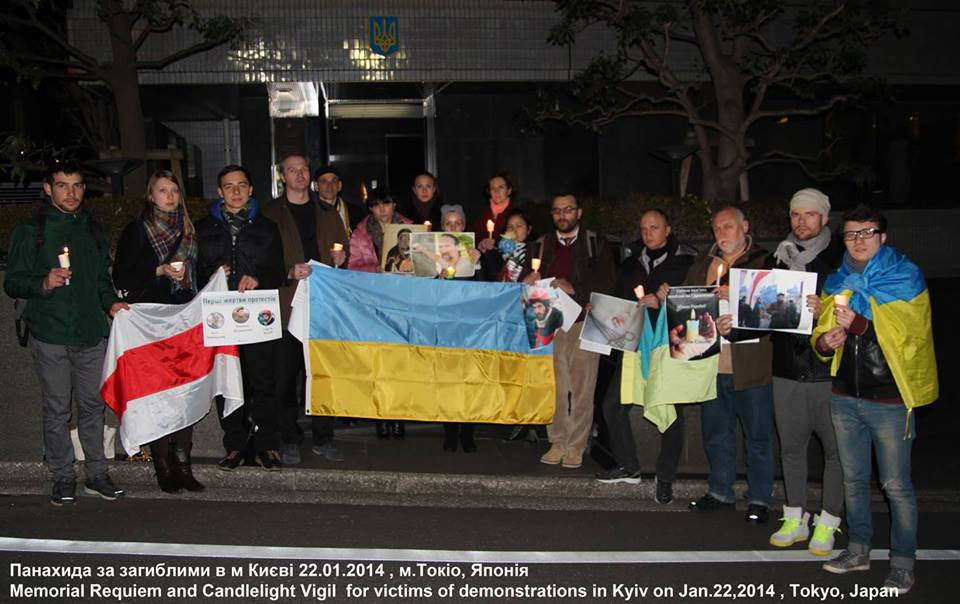
\includegraphics[width=0.8\linewidth]{images/molytva-za-zagyblyh}
		\end{center}
''Якщо не ми, тоді хто? Якщо не зараз, то коли?'' - колись сказав президент США Джон Кеннеді. Вірні Місії Української Православної Церкви в Японії (Українська Православна Церква Київського Патріархату) разом з друзями різних віросповідань зібрались перед Посольством України в Японії для проведення спільної молитви за упокій душі Сергія Нігояна, Михайла Жизневського та Юрія Вербицького, перших жертв злочинної диктатури в Києві. Деякі з працівників Посольства, які були на роботі, також приєднались до нашої молитви. Частина служби транслювалась наживо на Громадському ТБ.

\vfill
\columnbreak
\NewsItem{Благодійний майстер клас з писанкарства}
\NewsAuthor{Токіо}
		\begin{center}
			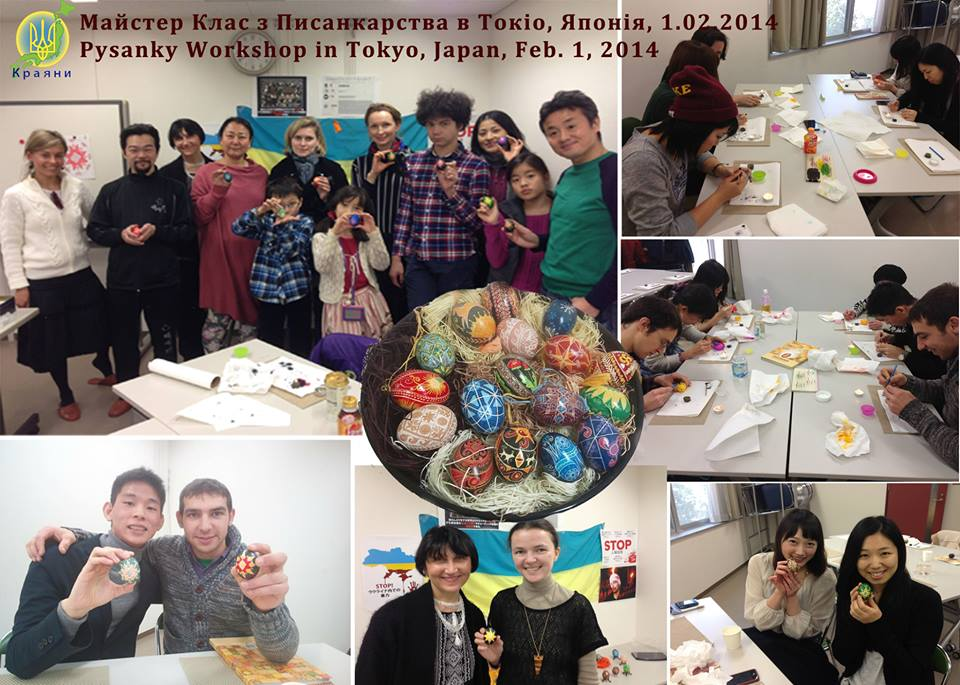
\includegraphics[width=0.8\linewidth]{images/pysankarstvo}
		\end{center}
1 лютого в Токіо відбувся благодійний майстер клас з писанкарства. 
Дякуємо всім, хто відгукнувся на наше запрошення і взяв участь у майстер класі. З вашою допомогою зібрано 61,000 ієн, які були відправлені на допомогу нашим постраждалим співвітчизникам.
		
\end{multicols}

\newpage

% Page 7
\Category{Українці в Японії}
\begin{multicols}{3}

\NewsItem{Концерт пам'яті жертв трагедії на АЕС Фукушіма}
\NewsAuthor{Кіото}
		\begin{center}
			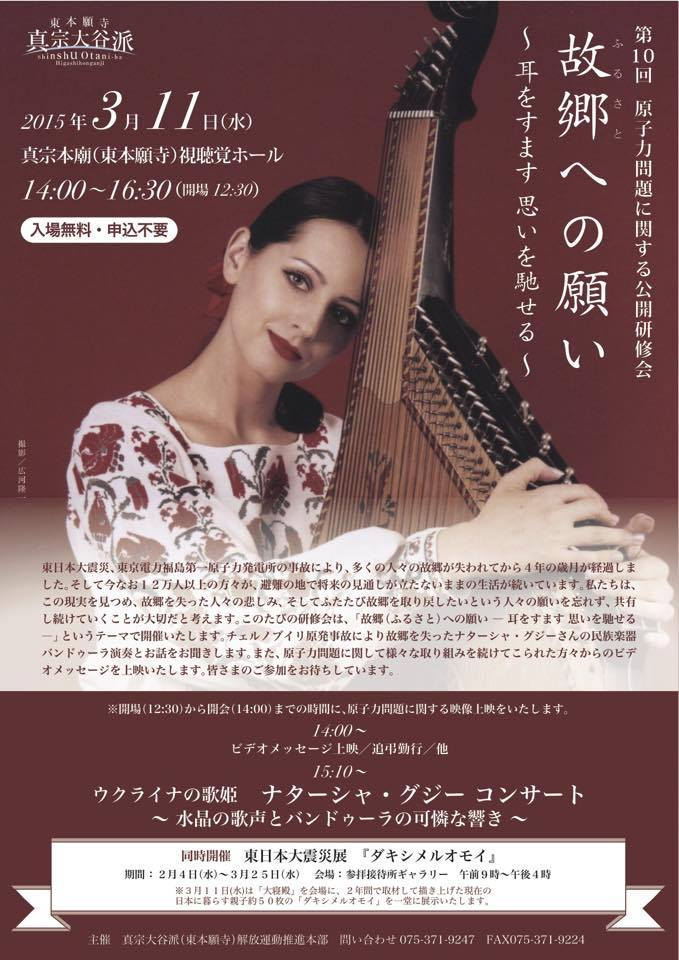
\includegraphics[width=0.8\linewidth]{images/concert-fukushima}
		\end{center}
В 4-ту річницю трагедії на АЕС Фукушіма-1 в місті Кіото звучала українська бандура. 11 березня там відбувся захід, присвячений пам'яті загиблих та постраждалих внаслідок аварії на АЕС Фукушіма-1. Бандуристка Наталя Ґудзій виступила з українськими мелодіями та піснями, а також розповіла про загублені домівки українців після аварії на Чорнобильській АЕС.

\vspace{1cm}
\NewsItem{Українське мистецтво в Японії}
\NewsAuthor{Фуджіока}
		\begin{center}
			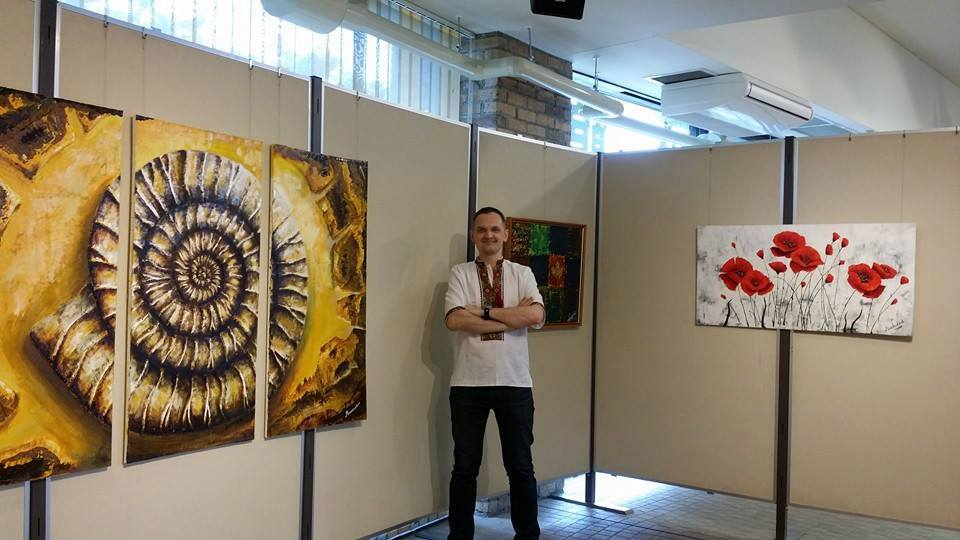
\includegraphics[width=0.8\linewidth]{images/mischak}
		\end{center}
Перша виставка картин українського митця в Японії Андрія Міщака відкрилась у місті Фуджіока, префектура Ґунма.

\vspace{4cm}
	\NewsItem{Вітаємо з перемогою!}
	\NewsAuthor{Москва}
		\begin{center}
			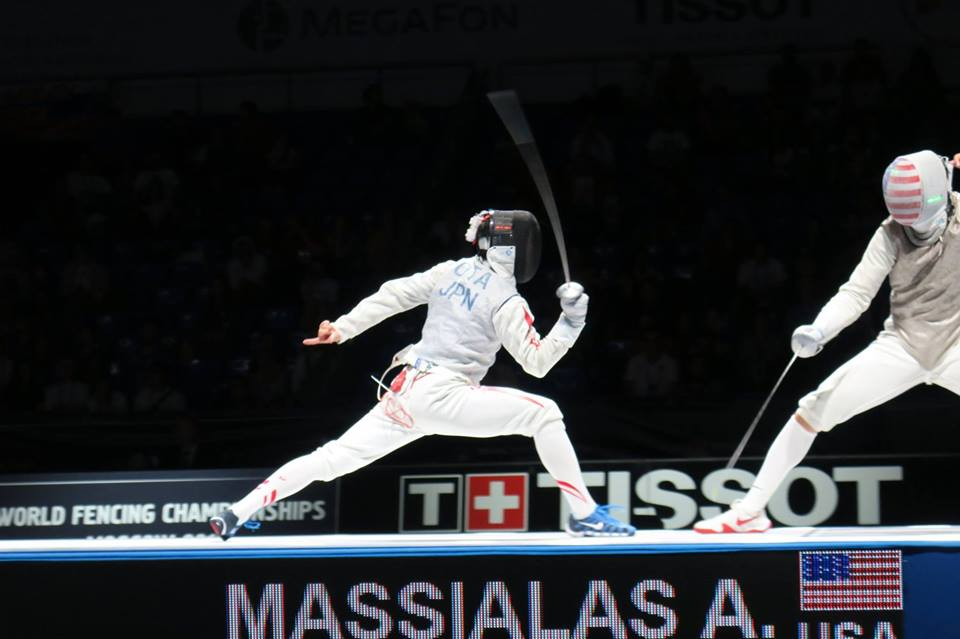
\includegraphics[width=0.8\linewidth]{images/rapiry}
		\end{center}
Вітаємо Олега Мацейчука - українця, головного тренера з фехтування на рапірах Японії, з перемогою вихованця, чемпіона світу з фехтування Юкі Ота (Японія). 
У фіналі чемпіонату світу серед чоловіків у двобої з американцем переміг японець. Золото з фехтування на рапірах стало першим в історії Японії.
Олег Мацейчук - киянин, екс-фехтувальник збірної України. В 2003 розпочав роботу тренером з фехтування в Японії. За період перебування в Японії виховав ціле покоління спортсменів, які вже самі стали тренерами.
Успіхів та нових досягнень!

\vspace{1cm}
\NewsItem{Майстер-клас з української кухні}
\NewsAuthor{Акаші, Хьоґо}
		\begin{center}
			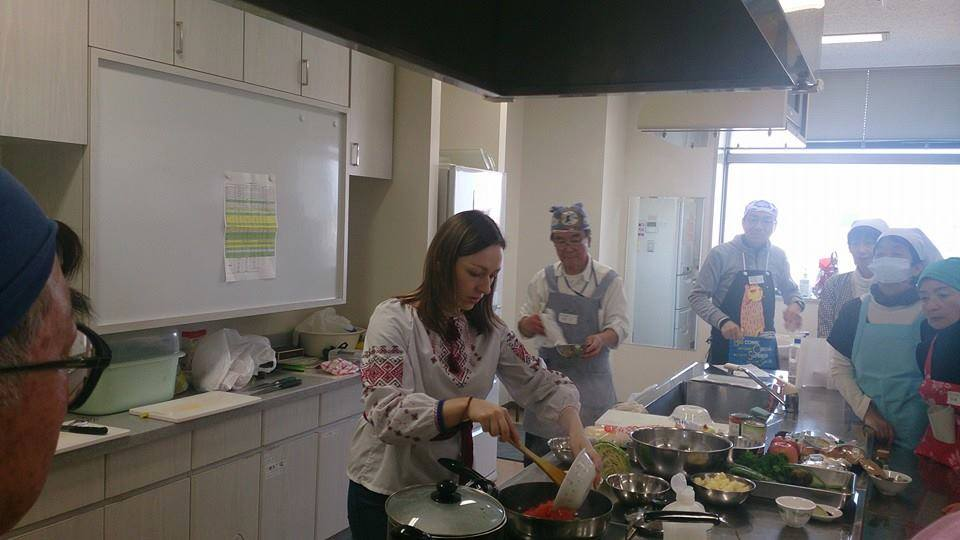
\includegraphics[width=0.8\linewidth]{images/ukr-cuisine-akashi}
		\end{center}
В місті Акаші, префектура Хьоґо, 4 березня відбувся майстер клас з приготування українських страв. За ініціативи Міжнародної асоціації міста Акаші Ольга Балинська та ще 20 містян зібрались на український обід. Навчались готувати український борщ, млинці з грибами та яблуками та салат з крабовими паличками. По обіді гостя заходу розповіла про Україну, кухню та вишиванки. Всім японським учасникам борщ та страви були до смаку і вони вже чекають наступного разу!

\vspace{1cm}
\NewsItem{Український вечір}
\NewsAuthor{Канаґава}
		\begin{center}
			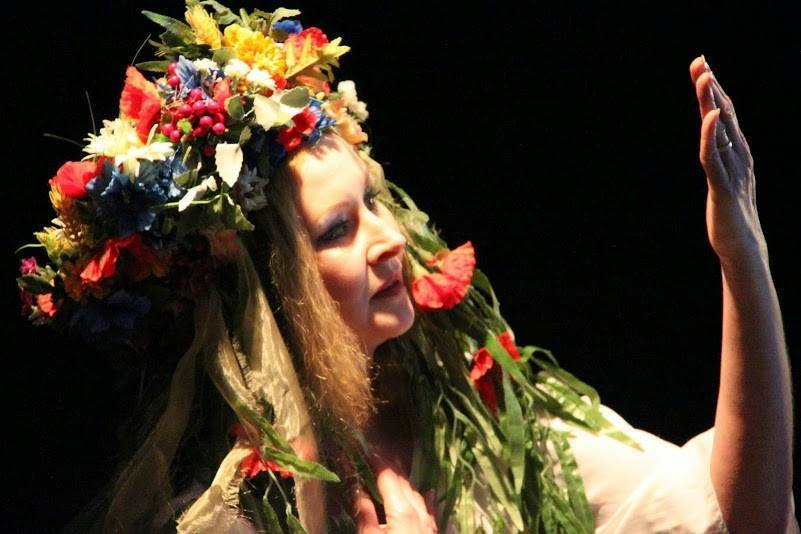
\includegraphics[width=0.8\linewidth]{images/ukr-evening}
		\end{center}
Вдруге в Японії, 22 лютого, в залі ГО ''Японія-країни Євразії'' у префектурі Канаґава відбувся ''Український вечір'' в рамках якого була виконана моновистава ''Княжна'' (за поемами Т.Г.Шевченка ''Відьма'', ''Княжна'') у виконанні Наталі Морозової-Шімади, переклад Оксани Піскунової, а також презентація України, її культури та звичаїв Оксаною Свистак.

Всіх присутніх вітала виставка старовинних українських книг, предметів побуту, вишиванок та рушників. Оксана Свистак розпочала вечір презентацією про Україну. Вихованка української школи в Токіо ''Джерельце'' Юлія привітала всіх присутніх чарівною піснею. У продовження вечора на всіх чекала вистава ''Княжна''. Наталя Морозова-Шімада виконувала виставу українською мовою, однак на екрані слова акторки дублювались японським перекладом, даючи змогу всім присутнім відчути силу Шевченкового слова.

Захід відвідали багато японців, кому цікава та небайдужа Україна, її культура та звичаї: студенти, працівники компаній, дослідники, духовенство. Під час прес-конференції присутні гості та представники ЗМІ задавали питання про українські вареники, жанр спектаклю, ситуацію в Україні, відомих українців та цікавились наступними подіями пов'язаними з Україною в Японії.

Фото: Юрій Свистак, Katsutaro Alexy Hirayama, Naoya Sakurai
\end{multicols}

\newpage

% Page 8
\Category{Цікавинки}

\begin{center}
\NewsItem{Патріотична кава}	

\includegraphics[width=0.6\textwidth]{images/kava}
\end{center}
В японських кав'ярнях українців зустрічають патріотичною кавою. В одній із кав'ярень в Токіо українців пригощали кавою, прикрашеною українським прапором та написом "Україна", а також тризубом. Таке оформлення не лише здивувало, але й підняло настрій українцям.
\SepRule	
\begin{multicols}{3}

\NewsItem{Миру Україні!}
\NewsAuthor{Танабата 2015}
		\begin{center}
			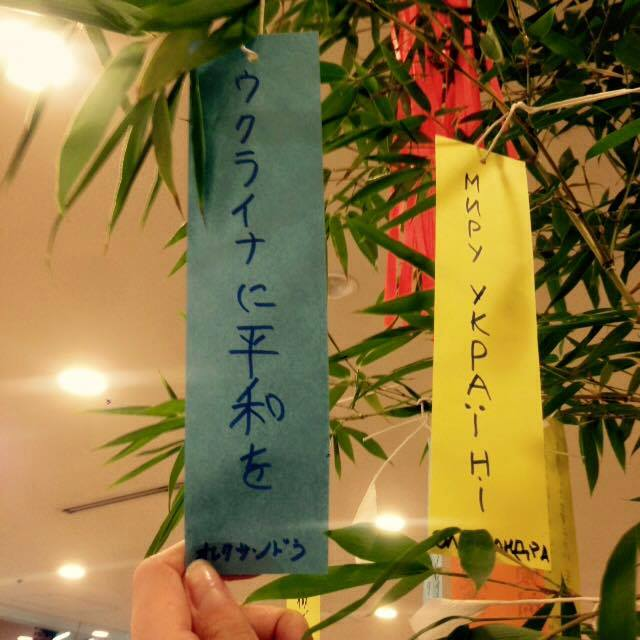
\includegraphics[width=0.8\linewidth]{images/tanabata}
		\end{center}
Побажання українців Японії на фестивалі Танабата. Японці вірять, що якщо 7-го липня написати своє бажання, то воно обов'язково здійсниться!

\vspace{1cm}
\NewsItem{Токійський Козак}
\NewsAuthor{Токіо}
		\begin{center}
			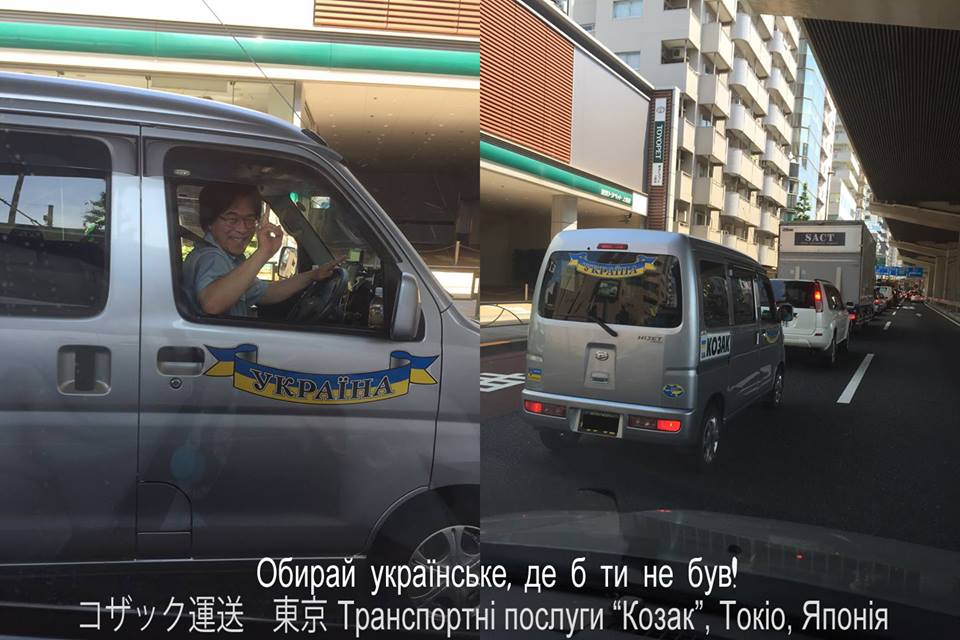
\includegraphics[width=0.8\linewidth]{images/kozak}
		\end{center}
Обирай українське, де б ти не був! Японці вражають своєю любов'ю до України та українського. Їдучи у справах по дорозі в Токіо українка почула сигнал іншого авто. Спочатку подумала, що вона порушила правила і за це їй сигналять. Її обганяє японець і з щасливою японською посмішкою вказує на свою машину, де наклейки з написом ''Україна'' та ''Козак'' та на її, де зображений український прапор. Так знаходять нових друзів по авто. Користуйтесь транспортними послугами ''Козака''! 

\end{multicols}

\newpage

% Page 9
\Category{Українські Свята}
\begin{multicols}{3}

\NewsItem{Христос Воскрес!}
\NewsAuthor{Великдень 2015}
		\begin{center}
			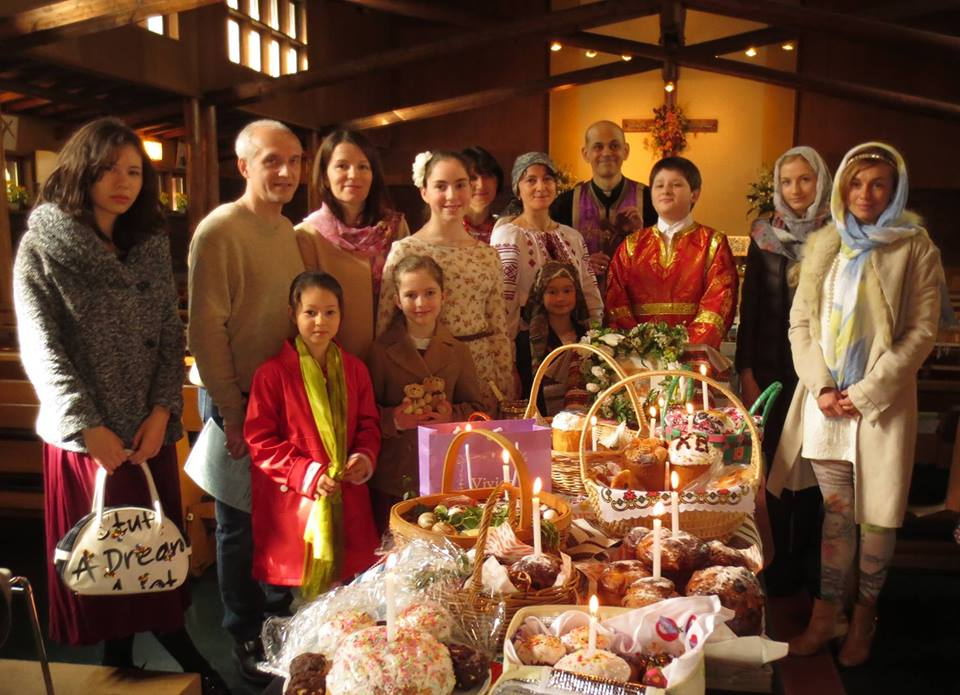
\includegraphics[width=0.8\linewidth]{images/paska}
		\end{center}
Українська громада Японії відсвяткувала Великдень в українській церкві в Токіо, після чого був організований святковий пікнік у колі друзів.

\vspace{1cm}
\NewsItem{Як українська громада відсвяткувала Святвечір та Різдво 2015 року в Японії}
\NewsAuthor{Токіо}
		\begin{center}
			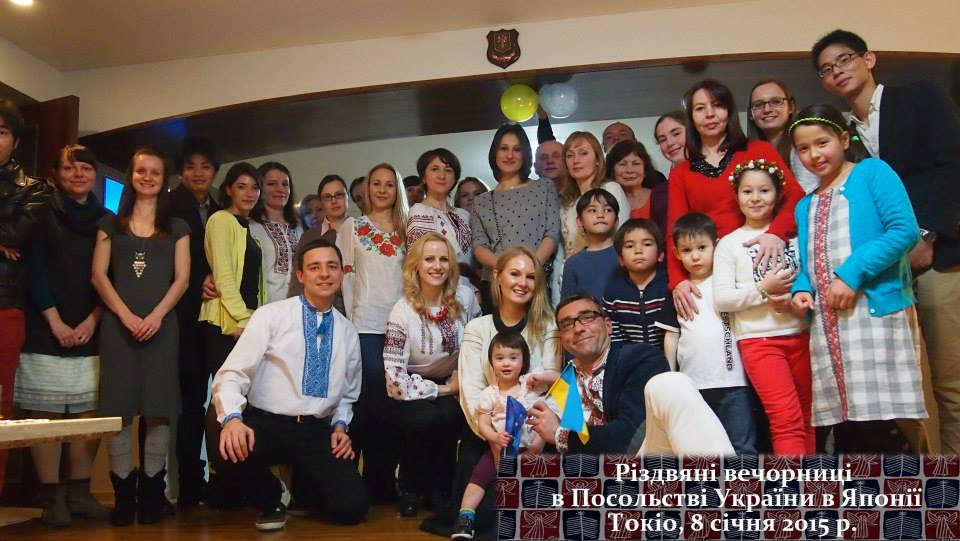
\includegraphics[width=0.8\linewidth]{images/rizdvo}
		\end{center}
У Святвечір 6 січня українці та японські друзі в Токіо зустріли зорю на вечірній службі місії Української Православної Церкви Київського Патріархату (St. Jude Ukrainian Orthodox Mission, Tokyo) та зібрались за Святою Вечерею.
А на Різдво громадою колядували у Посольствi України в Японії, де всіх гостинно приймав Посол Ігор Харченко разом зі своєю дружиною, донькою та усім дипломатичним корпусом Посольства. Збирали благодійну допомогу захисникам України.
Вперше за роки незалежності ''українська хата'' в центрі Токіо вітала громаду українців та друзів у своїх стінах на Різдвяних вечорницях. За давніми традиціями колядники віншували господарів Амбасади колядкою ''Добрий вечір тобі, пане господарю'', а опісля Посол привітав усіх гостей.
У своєму вітальному зверненні Посол познайомив всіх гостей з нечисленним, але дружнім колективом дипломатичної установи та запросив всіх звертатись до її працівників. Оскільки Посольство України в Японії - це ''українська хата, то до хати мають приходити люди''. Посол подякував всій громаді за підтримку протягом минулого року, побажав миру, злагоди та сподівається на подальшу співпрацю громади та Посольства у спільній справі.
Святковий стіл вітав присутніх українськими варениками, млинцями та іншими стравами, до приготування яких долучились як господарі дому, так і українські господині Японії. Всі охочі могли скуштувати українських кримських вин.
Вечір був наповнений радості, злагоди, надії на мир та спокій в Україні, у кожній родині. Усі присутні разом виконали колядки ''Нова радість стала'', ''Добрий вечір тобі, пане господарю'' та щедрівку ''Ой, сивая тая зозуленька''.
10 тисяч гривень було зібрано українською громадою на підтримку захисників України в Різдвяний вечір у Посольстві, а також під час інших новорічних заходів українців в Японі.
Дякуємо Посольству та всім причетним до організації та проведення заходу за чудовий вечір!
Христос народився! Славімо Його!
Слава Україні!

\vspace{1cm}
\NewsItem{Шевченківські читання в Японії}
\NewsAuthor{Токіо, Хараджюку}
		\begin{center}
			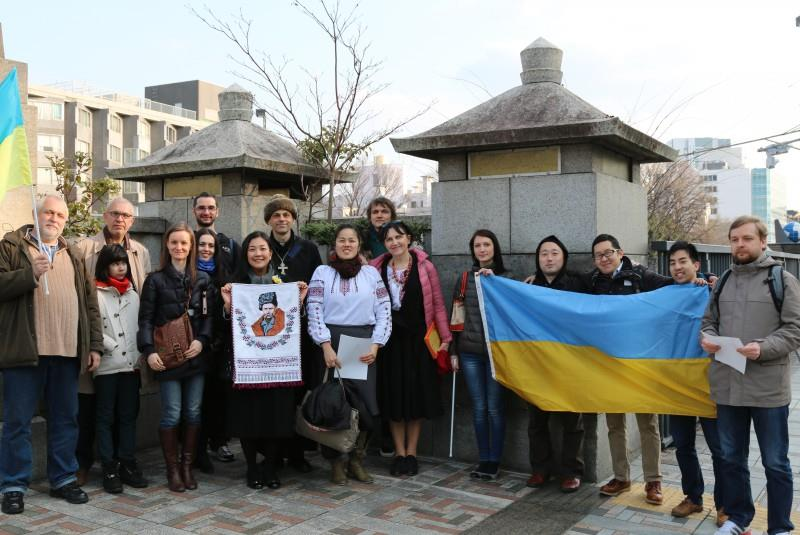
\includegraphics[width=0.8\linewidth]{images/shevchenko-reading}
		\end{center}
9 березня, до дня народження великого Кобзаря відбулись читання творів Тараса Шевченка біля станції Хараджюку в Токіо, напроти головного входу до Парку Мейджі. Українська громада в Токіо приєдналася до глобальної акції ''Світ читає Шевченка''. 
Звучав ''Заповіт'', ''Садок вишневий коло хати'' та інші твори пророка українською та японською мовами. 
У всесвітній акції взяло участь більш ніж 30 населених пункти в Україні та 22 країни по всьому світу.

\end{multicols}

\newpage

% Page 10
\Category{Українська Недільна Школа ''Джерельце''}
\begin{multicols}{3}

\NewsItem{Ласкаво просимо до ''Джерельця''!}
\NewsAuthor{Токіо}
		\begin{center}
			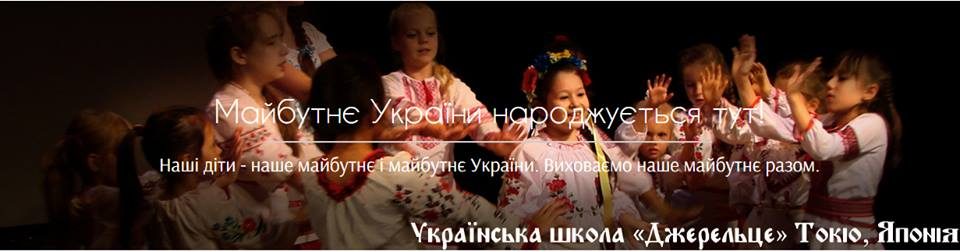
\includegraphics[width=0.8\linewidth]{images/dzherelce}
		\end{center}
Українська школа для дітей "Джерельце" в Токіо запрошує дітлахів на навчання! Подробиці щодо діяльності школи, розкладу занять та інша інформація - на сайті http://dzherelce.github.io/

Українська школа для дітей розпочала свою роботу у березні 2009 року. Головною метою школи є навчити дітей українських та багатонаціональних родин розуміти та спілкуватись українською мовою, познайомити з дитячим фольклором, українською культурою, підтримувати та зберігати традиції свого народу.

Професійні вчителі навчають малят читанню, письму, математиці, мистецтву. Разом з батьками і вчителями вихованці знайомляться з традиціями Батьківщини, готують новорічні та Великодні вистави, Різдвяні вертепи, навчаються розписувати писанки на Великдень. Вихідні проводять в захоплюючих походах у гори або у літньому таборі. Майбутнє України народжується тут!

\vspace{1cm}
\NewsItem{''Івасик Телесик'' в Японії}
\NewsAuthor{Токіо, школа ''Джерельце''}
		\begin{center}
			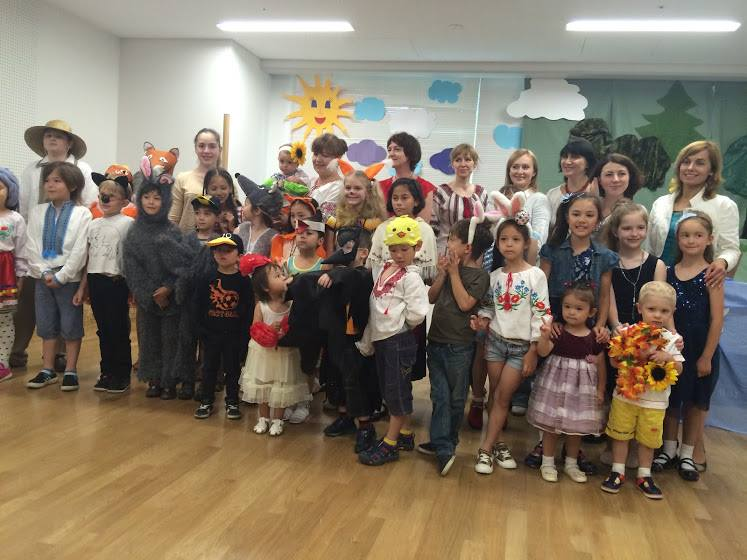
\includegraphics[width=0.8\linewidth]{images/telesyk}
		\end{center}
''Івасик Телесик'' в Токio на останньому уроці недільної школи Джерельце 14 червня. В День ''останнього дзвоника'' японського Джерельця вихованці школи порадували батьків та вчителів виставою, за казкою ''Івасик Телесик''. За успіхи у навчанні учні отримали вітальні грамоти та подарунки. Українська дитяча школа ''Джерельце'' була заснована у березні 2009 року в місті Токіо. Заняття в школі проводяться двічі на місяць кваліфікованими вчителями за власно розробленою програмою. Сьогодні кількість вихованців нараховує більше 40 учнів різних вікових категорій. Дітлахи мають змогу навчитись читанню, письму, математиці та мистецтву. Діти знайомляться з традиційними святами, готують Новорічні та Великодні вистави, Різдвяні Вертепи. Отримати більше інформації та записатись на заняття можна на сайті школи dzherelce.github.io

\vspace{1cm}
\NewsItem{День Знань}
\NewsAuthor{Токіо, Школа ''Джерельце''}
		\begin{center}
			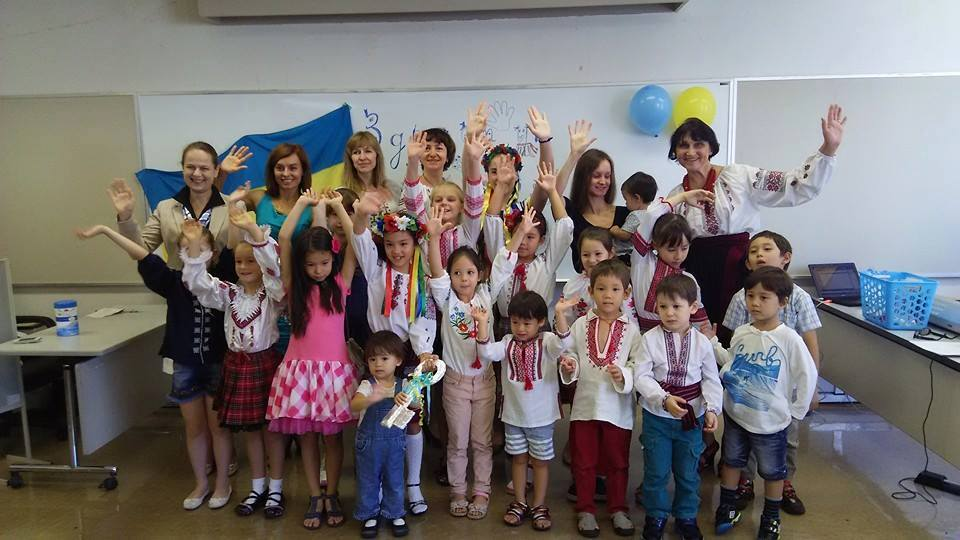
\includegraphics[width=0.8\linewidth]{images/den-znan}
		\end{center}
Так пройшов День Знань в недільній школі ''Джерельце'' 2014 року.

\end{multicols}

\newpage

% Page 11
\begin{center}
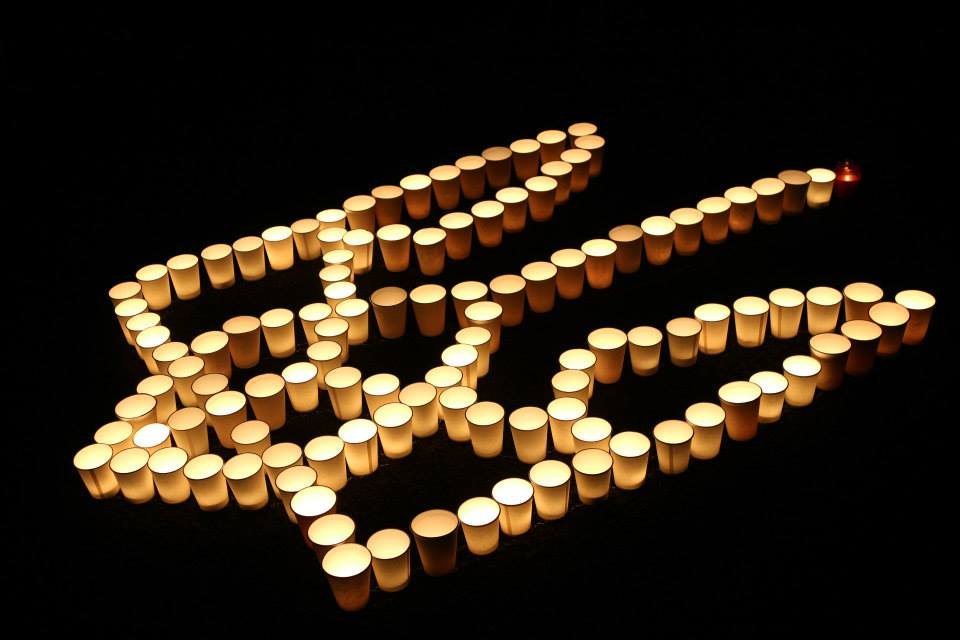
\includegraphics[width=0.8\linewidth]{images/tryzub}
\SepRule			
Цей випуск Часопису присвячується всім загиблим від російської агресії на Сході України.
\end{center}

\end{document} 
